% Self-contained local starter inspired by the NTNU Laboratory Report in Physics
% template by Vebjorn S. Forde (CC BY 4.0):
% https://www.overleaf.com/latex/templates/ntnu-laboratory-report-in-physics/zrkxstqtpdpv
% This is a simplified adaptation, not the original multi-file project.
% Compile with pdfLaTeX in TeXstudio. Replace the example text and metadata.

\documentclass[5p,a4paper]{elsarticle}

\usepackage{pdfpages}

% Common TeX Live packages
\usepackage[utf8]{inputenc}
\usepackage[T1]{fontenc}
\usepackage[english]{babel}
\usepackage{lmodern}
\usepackage{geometry}
\geometry{margin=25mm}
\usepackage{microtype}
\usepackage{graphicx}
\usepackage{amsmath,amssymb}
\usepackage{siunitx}
\usepackage{booktabs}
\usepackage{float}
\usepackage{caption}
\usepackage{enumitem}
\usepackage[hidelinks]{hyperref}
\usepackage[numbers]{natbib}

% ---------- Report details: edit these ----------
\newcommand{\reporttitle}{Uniaxial Tensile Test of Polycarbonate with DIC}
\newcommand{\course}{Modern Experimental Mechanics}
\newcommand{\studentname}{Vilmer Dahlberg}
\newcommand{\studentid}{}
\newcommand{\labdate}{2026/11/05}
\newcommand{\submissiondate}{\today}
\newcommand{\institution}{Department of Construction Sciences,  Lund University}

%----------------------------------------------------------
% Math macros
%----------------------------------------------------------
\usepackage{amsmath,amssymb,amsfonts}%
\usepackage{tensor}
\usepackage{upgreek}
\usepackage{sansmath}
\usepackage{xspace}
\usepackage{array}
\usepackage{mathtools}
\newcommand{\bm}[1]{\text{\boldmath{$#1$}}}

\graphicspath{{../results/}, {../figures/}}

\begin{document}
	
	\begin{frontmatter}
	
		\title{\reporttitle}
		\author{\studentname}
		\address{\course\\\institution}
		
		\begin{abstract}
			
		\end{abstract}
		
		\begin{keyword}
			DIC \sep polycarbonate \sep figure
		\end{keyword}
	
	\end{frontmatter}
	
	\section{Introduction}
	This report is concerned with the digital image correlation (DIC) of a polycarbonate sample subject to uniaxial tension. This is an extension of a previous experiment in which only the force-displacement data was analyzed. To avoid repeating myself i will refer to the report, found in \ref{app:report1} for an introduction to the experiment.
	
	
	% Introduction to DIC
	As mentioned in the previous report, the force-displacement data gathered via the strain gauge does not contain any information about the local deformation of the sample. Since we're considering deformable bodies, and not rigid bodies, the deformation state in the sample will vary throughout it's geometry. Thus we require full-field measurements of the deformation state if we want to be able to analyze the material behavior.
	
	Full-field measurements are roughly divided into destructive and non-destructive methods \textcolor{red}{ref to something here}, of which photo-DIC \textcolor{red}{what's this actually called?} is a common non-destructive alternative. Partially due to its ease of use, at least compared to alternatives such as X-ray or neutron tomography. 
	
	% Intro should not explain the method, maybe just compare some popular DIC methods and discuss local versus global and incremental versus cumulative DIC
	
	% in-situ????
	
	%
	In 2D camera-DIC, the sample is imaged throughout the experiment. As a post-processing step, the images are 
	
	% how do you even explain DIC?
	
	% something about the speckle pattern
	
	% something about comparing small regions at a time (local DIC)
	
	% 
	Additionally, to be able to compare image segments in the proceeding DIC step the sample must have a texture on its surface. 
	
	
	To perform 2D camera-DIC we 
	
	\section{Method}
	
	\subsection{Experimental setup}
	In this experiment we use the same method as in the previous experiment, except we add both a camera and lighting equipment to capture images of the sample throughout the tensile test.
	
	
	We begin by applying a texture to the sample, which in this experiment consists black ink sprayed over the specimen's surface.
	
	The camera (dector) is mounted in front of the sample. To illuminate the sample, a light is placed to the right of the camera, as per Figure \ref{fig:method:experimental_setup}.
	
	\begin{figure}
		\centering
		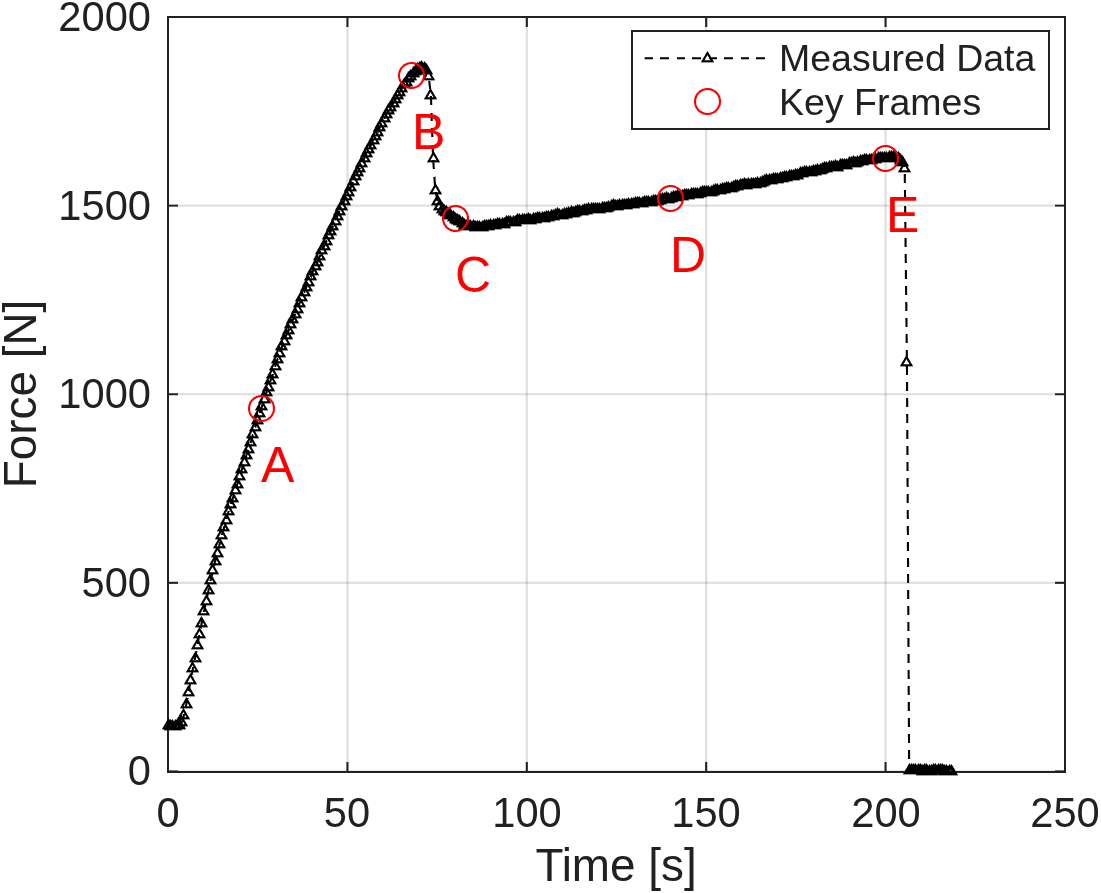
\includegraphics[width=\linewidth]{force_disp.png}
		\caption{Experimental setup.}
		\label{fig:method:experimental_setup}
	\end{figure}
	
	
	% After the experiment part, how the DIC is actually performed. 
	
	% Note about sampling frequency of load cell
	
	% Note about sampling frequency of camera
	
	\subsection{DIC}
	
	% Correlation function
	Before discussing correlation functions, its worth revisiting the definition of the angle $\theta_{uv} \in [0,\,\pi/2]$ between two vectors $u,\, v \in \mathbb{R}^n$, given by
	\begin{equation}
		f_{cc}(u, v) = \frac{u\cdot v}{||u||_2 ||v||_2} = \cos{\theta_{uv}}
	\end{equation}
	If two vectors $u$ and $v$ are orthogonal, then their inner product is zero and hence $\theta = \frac{\pi}{2}$. On the other hand, if they are parallel, then $\cos{\theta} = 1$, and hence $\theta=0$. The loss function used in this experiment is the zero-normalized cross-correlation (ZNCC) \textcolor{red}{ref to this}, which is related to the cosine of the angle. Given two images $F,\,G \in \mathbb{R}^{n\times n}$, the ZNCC is defined by
	\begin{equation}
		l_{ZNCC}(F, G) = f_{cc}(\textsc{FL}(F) - \mu(F), \textsc{FL}(G) - \mu(G))
	\end{equation}
	where $\textsc{FLAT}(X)$ flattens the $n\times n$ image $X\in \mathbb{R}^{n\times n}$ to the vector $x\in \mathbb{R}^{2n}$ and $\mu(x)$ computes the mean value of $x$. 
	
	% Subpixel refinement
	In local DIC, for each strain measurement, we take a reference image $\mathcal{F}$ and the current image $\mathcal{G}$. We then proceed by considering one region of the specimen at a time, represented by the motif $\mathcal{M}\subset\mathcal{F}$. To compute the displacement of points near the region of interest, we compare $\mathcal{M}$ with equally sized regions sub-regions $\mathcal{H}$ of $\mathcal{G}$. For each subregion $\mathcal{H}$ the loss $l$, in this case $l_{ZNCC}$, is evaluated and stored. The $\mathcal{H}$ for which the loss attains it's maximum defines the displacement of the original region of interest.  
	
	In practice, the displacement of any region of the sample may take on any finite displacement. In fact, it may also rotate and warp. However, in comparing sub-regions of the \textit{images}, the displacement may only be an integer multiple of the pixel size in any given direction. Thus using the outlined approach, in the best case we get a rounding error of the displacements. The strain fields, which are gradients of the displacements, may have very large jumps in regions where the actual displacement modulo the pixel size is close to $0.5$ pixel sizes, or very small gradients in regions where the actual displacement modulo the pixel size is close to $0$. This is not a new problem, common remedies are interpolation of the output or input, or so-called optical flow.
	
	In interpolating the input, we let the displacements be real numbers and pose the cross-correlation search as an optimization problem, which can be solved with gradient descent. When evaluating the cross-correlation we require an subpart of the image, which is given by interpolating the image given the displacement. \textcolor{red}{refine this statement}. The benefit to this method is that any model of the deformation can be built, which allows for stretches and rotations, for example. This does lead to a somewhat more complex implementation, however. 
	
	In interpolating the output, we proceed as before, but once all the grid-points have been considered, we build an interpolation of the cross-correlation which spans not only the integers but also the in-between real values, and minimize the loss over those values. The benefit being it's relatively simple.
	
	In practice, we expect that the displacements of points should be local, meaning we restrict the search to a subwindow of the current image.
	
	The DIC algorithm implemented for this experiment is based on image interpolation. Inter-pixel values are found by interpolating neighboring images, with lagrange polynomials. The displacements are found by using a simplex optimization algorithm, which is gradient-free. Due to it's sensitivity of initial guess, we choose the last displacement value as initial guess, if the loss is high enough. Otherwise, we use find an initial guess using loss-interpolation. The algorithm is described in
	
	% algorithm descrption
	
	Finally, to compute the displacement gradients we use a central difference scheme, i.e.
	\begin{align*}
		\frac{\partial u_x^{i,j}}{\partial x} & \approx \frac{u_x^{i,j+1}-u_x^{i,j-1}}{2 \Delta x} \\
		\frac{\partial u_x^{i,j}}{\partial y} & \approx \frac{u_x^{i+1,j}-u_x^{i-1,j}}{2 \Delta y} \\
		\frac{\partial u_y^{i,j}}{\partial x} & \approx \frac{u_y^{i,j+1}-u_y^{i,j-1}}{2 \Delta x} \\
		\frac{\partial u_y^{i,j}}{\partial y} & \approx \frac{u_y^{i+1,j}-u_y^{i-1,j}}{2 \Delta y} 
	\end{align*}
	where $u_x^{i,j}$ and $u_y^{i,j}$ denote the measured displacements at pixel $i,j$ in the $x$ and $y$ direction, respectively. 
	
	% Principle strains and directions?
	
	% How to compute the pixel height and width.
	To compute relate the height and width the first image is read. 
	
	\section{Results and Discussion}
	The force-displacement graph is shown in figure \ref{fig:result:force_disp}. As performing the DIC for all frames would be excessive, only a few key frames, marked by red circles in the graph, are analyzed. The corresponding incremental principle strains and cross-correlation are shown in Figure \ref{fig:result:strain_interp_img}. 
	
	Starting with frame A, the strain field looks to be quite homogenous (at this scale) although there seems to be some concentration near the notch center. Also note the rather big estimated strains near the boundary. This is caused by the displacement effectively being zero outside the sample. 
	
	\begin{figure}
		\centering
		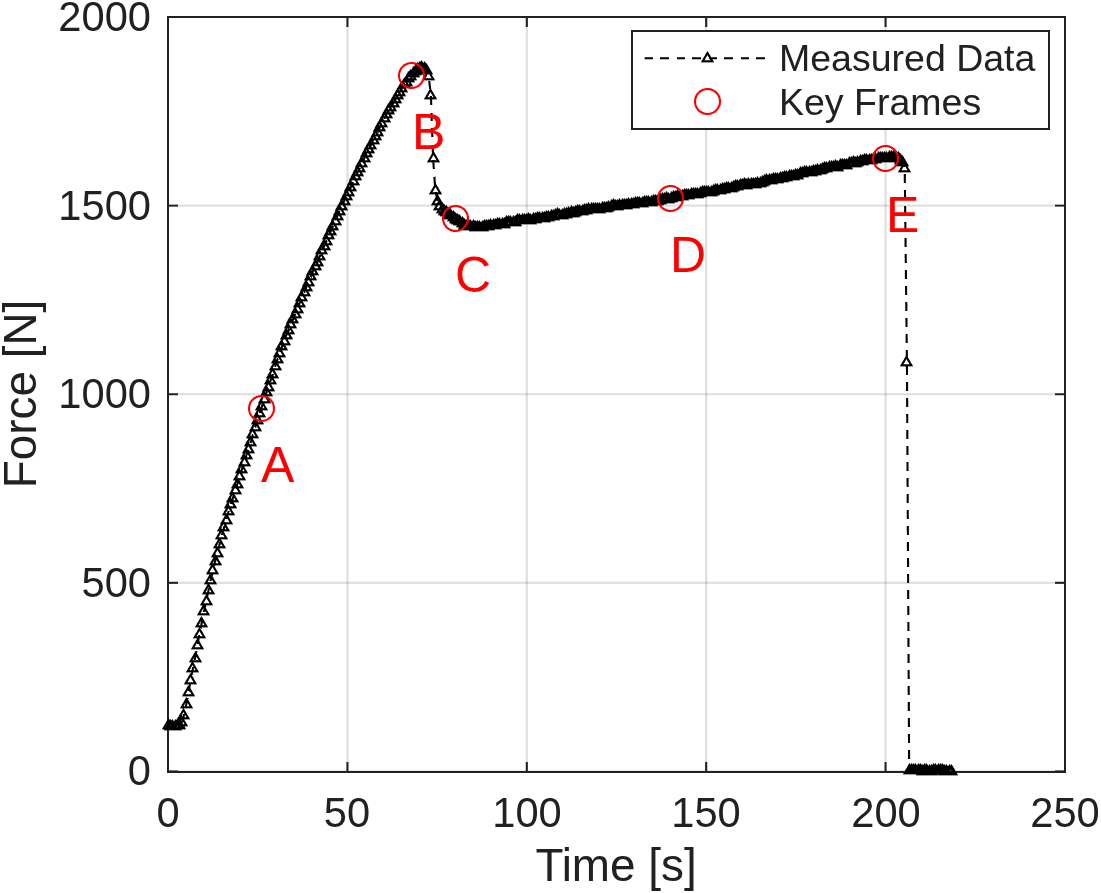
\includegraphics[width=\linewidth]{force_disp.png}
		\caption{Measured forces using the load cell over time.}
		\label{fig:result:force_disp}
	\end{figure}
	
	\clearpage
	\onecolumn
	\begin{figure}
		\centering
		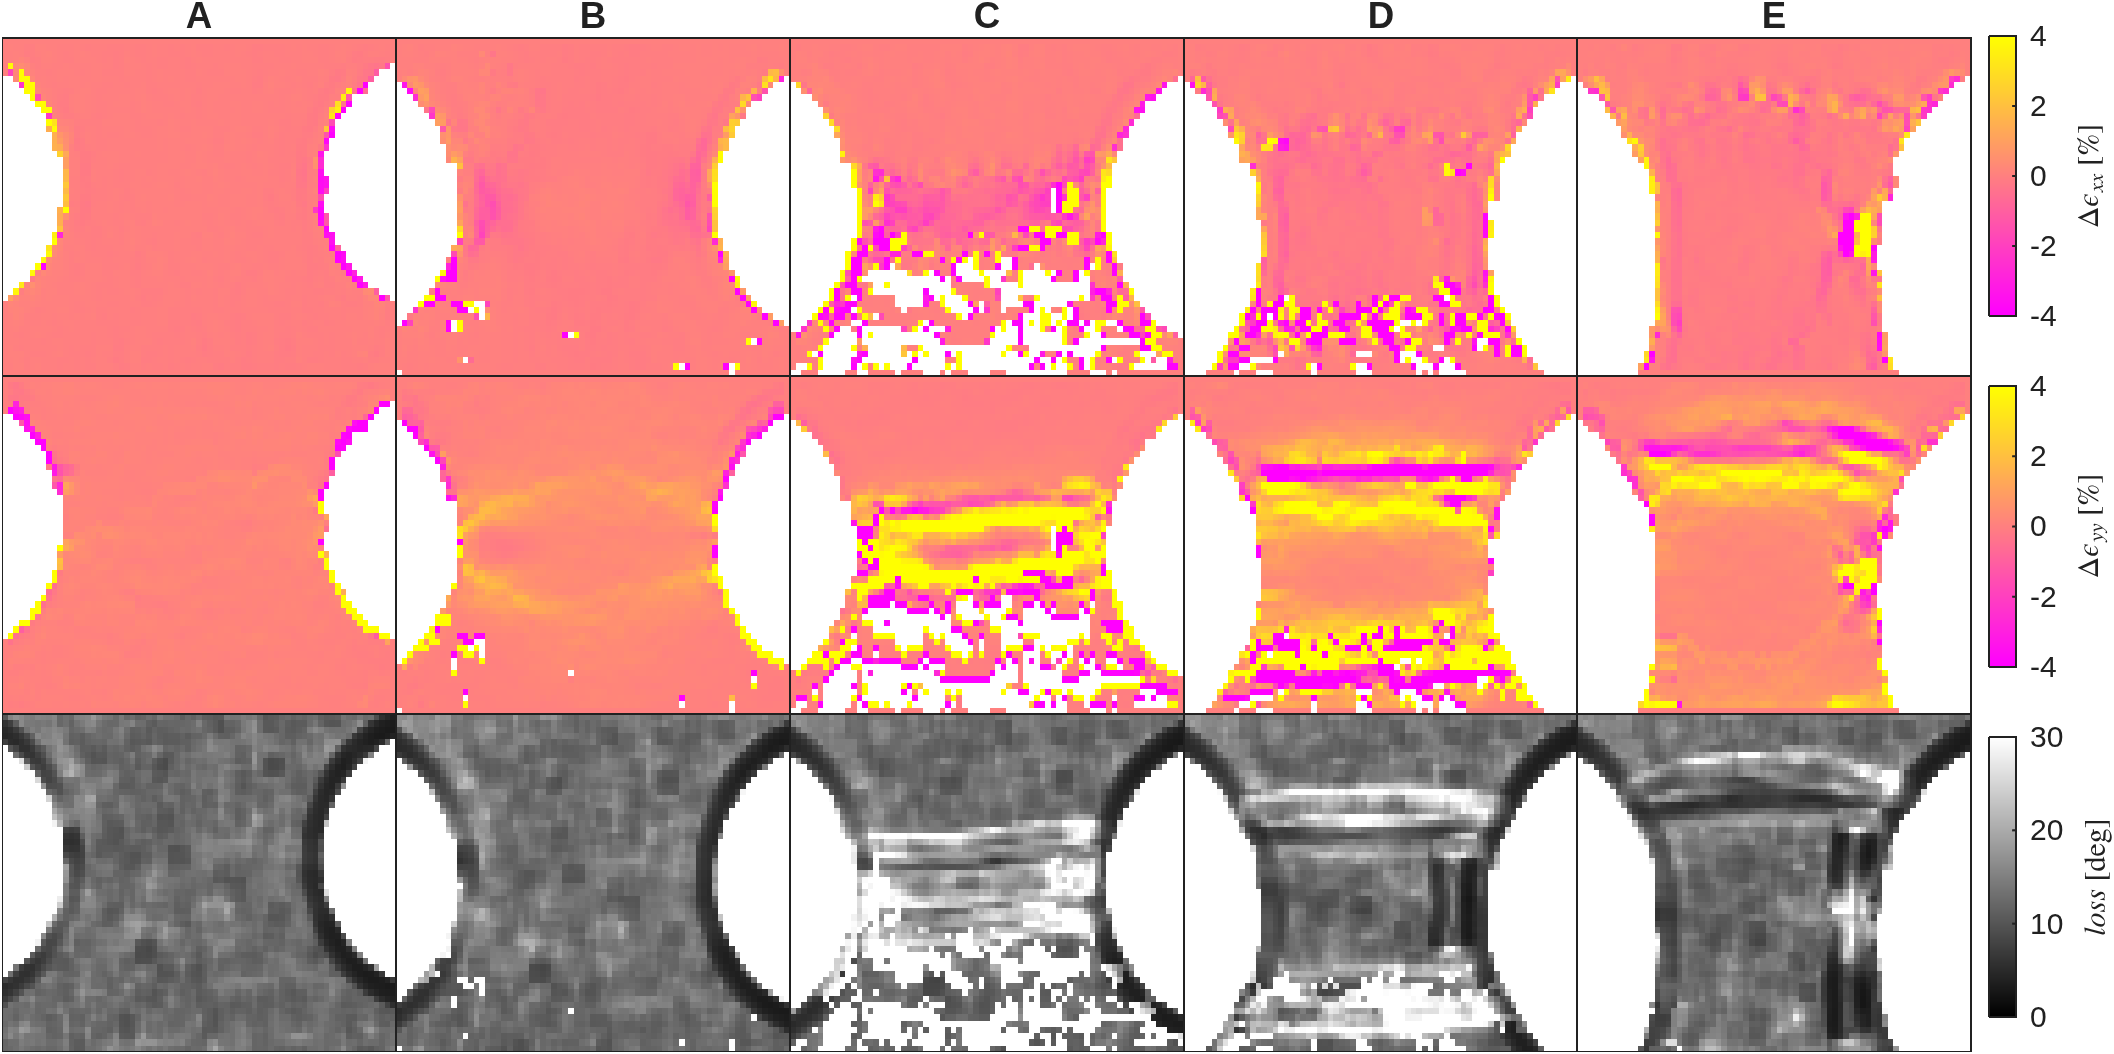
\includegraphics[width=\linewidth]{int_img_grid.png}
		\caption{Top two rows show the two principle strains. The third row shows the principle angle and the bottom row shows the loss (in radian). The background is filtered using a mask, based on a K-means clustering (k = 2) of the loss field.}
		\label{fig:result:strain_interp_img}
	\end{figure}
	
	\twocolumn
	
	\section{Conclusions}
	
	\bibliographystyle{unsrtnat}
	\bibliography{refs.bib}
	
	
	\clearpage
	\appendix
	\onecolumn
	\section{Uniaxial Tensile Test of Polycarbonate Sample} \label{app:report1}
	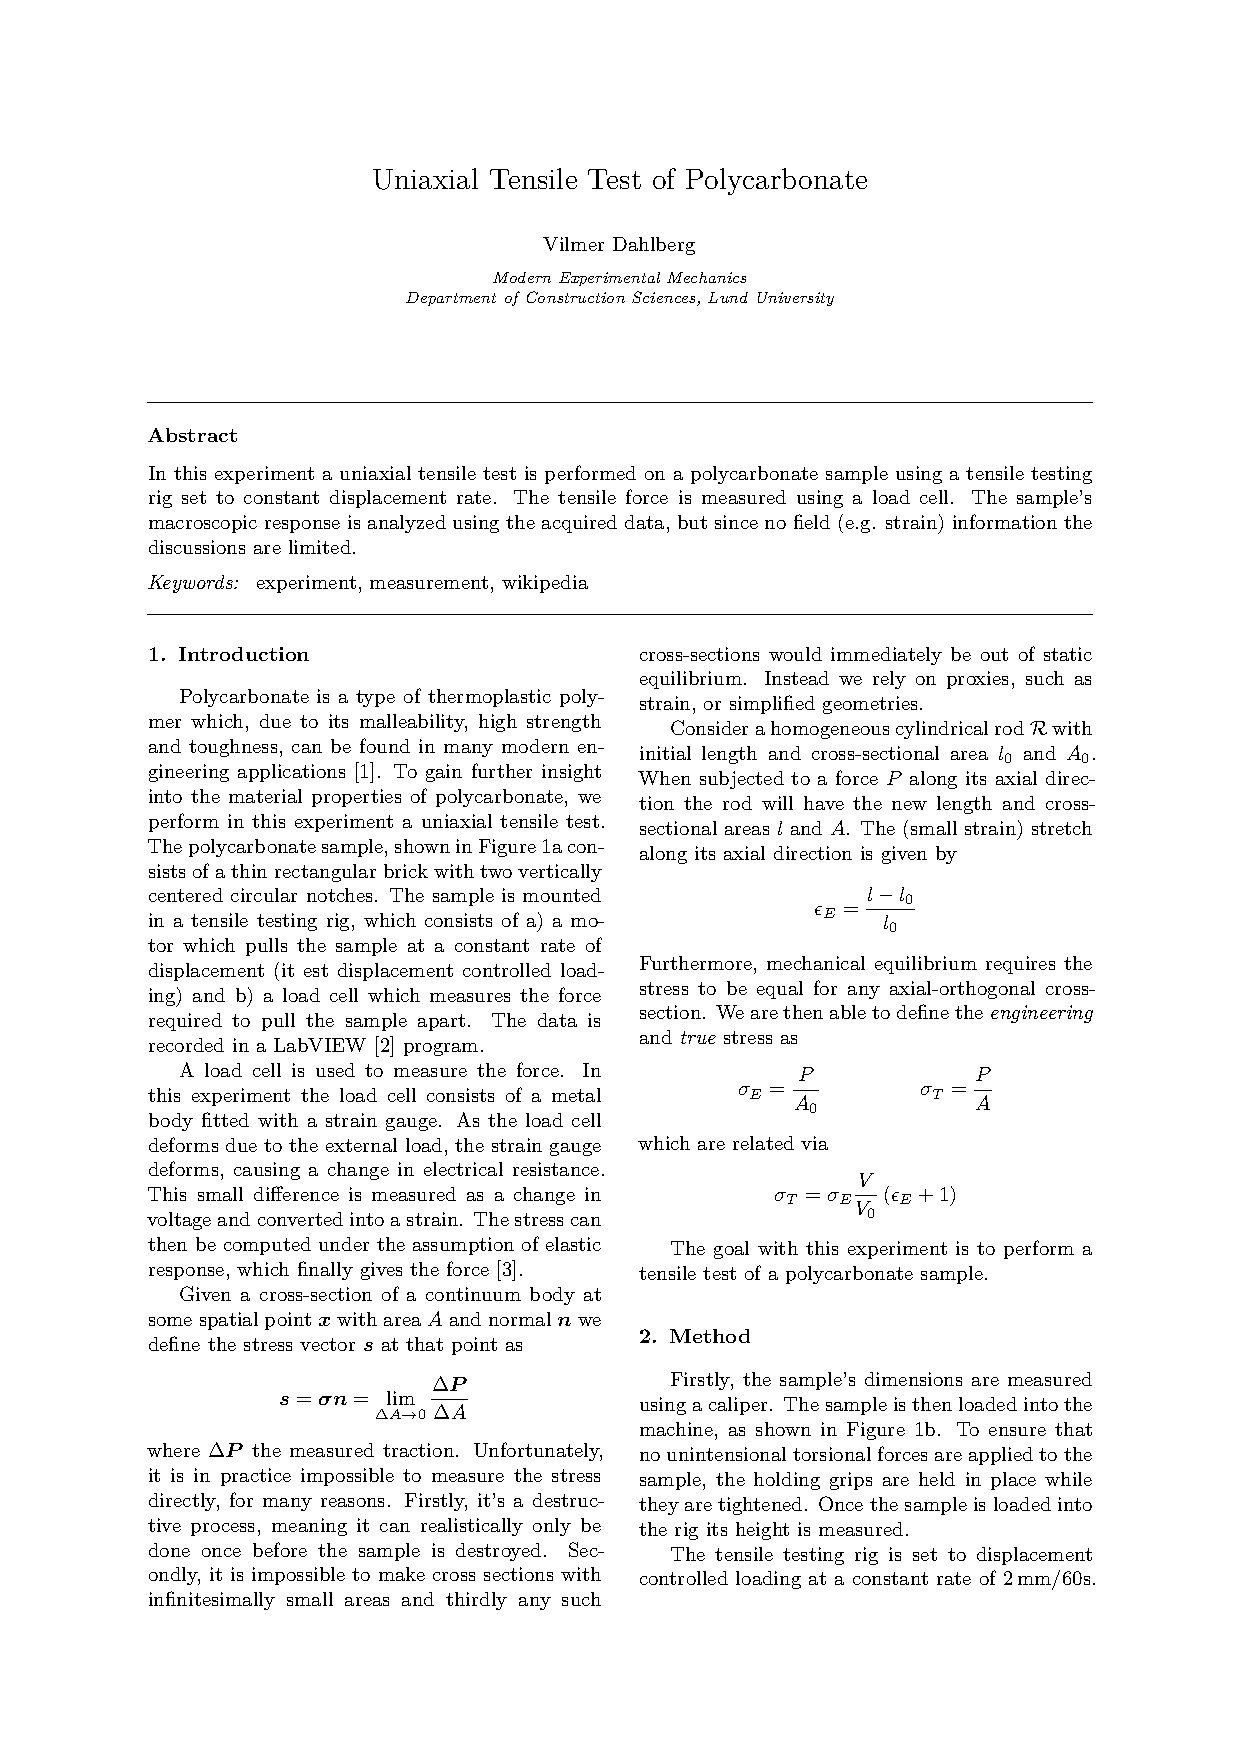
\includepdf[pages=-, pagecommand={}]{../../experiment1/manuscripts/main_simple.pdf}
	\twocolumn
	
\end{document}
